% ┌────────────────────────────────────────────────────────────────────────────┐
% │ NANOSTRING PAPER                                                           │
% │   Genetic instability and recurrent MYC amplification in ALK-translocated  │
% │   NSCLC: a central role of TP53 mutations                                  │
% └────────────────────────────────────────────────────────────────────────────┘

\chapter{Theragnosis Biomarkers in Lung Cancer}
\sectionmark{Theragnosis Biomarkers in Lung Cancer}

This study investigates the connection between rearrangement of the anaplastic
lymphoma kinase (\textit{ALK}) and \textit{TP53} mutations in human non-small
cell lung cancer.

Lung cancer, one of the main causes of death in humans \citep{Siegel2018}, is
traditionally divided into two types: small cell lung cancer (SCLC) and non-%
small cell lung cancer (NSCLC), which constitutes over \SI{80}{\percent} of
all cases \citep{Reck2014}. However, NSCLC has proven to be too diverse and is
now treated as a collection of many different cancer types that each require
individual treatment regimes \citep{Boolell2015}. One of these is \textit{ALK+}
lung cancer, in which the \textit{ALK} gene breaks and fuses with other genes
\citep{Holla2017}.

The \textit{ALK} gene encodes a receptor tyrosine kinase that is only expressed
in early embryonic development and is involved in cell proliferation, survival,
and differentiation of the nervous system \citep{Iwahara1997}.
% While the ligands of ALK are unknown, its downstream signalling pathways have
% been characterised \citep{Stoica2001,Stoica2002,Bennasroune2010,Murray2015}.
However, in \textit{ALK+} lung cancer, the fusion of \textit{ALK} to other genes
causes uncontrolled activation of its downstream signalling paths through the
fusion partner's promoter \citep{Holla2017}. In turn, tyrosine kinase inhibitors
(TKI) have been shown to be an effective treatment for \textit{ALK+} lung cancer
\citep{Kwak2010,Reck2014}.

\citet{Gainor2016} found that \SI{33}{\percent} of \textit{ALK+} tumours also
show mutations in the \textit{TP53} gene, and \citet{Aisner2018} discovered
that \textit{TP53} mutations reduced patient survival in \textit{ALK+} lung
cancer. \textit{TP53} is classified as a tumour suppressor gene, as it
prevents genome mutation \citep{Surget2013}. It plays a role in cell cycle
regulation and apoptosis, activating DNA repair mechanisms when damage has
been sustained and halting the cell cycle until the damage is repaired. If the
damage is too severe and cannot be repaired, it initiates programmed cell
death. \textit{TP53} mutations are thus frequent in many cancer types, as
inactivation of \textit{TP53} severely compromises tumour suppression \citep{%
Olivier2010}.

Our assumption, which we could corroborate in the publication, was that
mutations in \textit{TP53} lead to genetic instability, which in turn promote
the development of resistance mechanisms, reducing patient survival rate in
\textit{ALK+} lung cancer \citep{Alidousty2018}.

% \bigbreak
% \noindent

\subsubsection{Methodology}\label{subsubsec:alkmethod}
\addcontentsline{toc}{subsection}{Methodology}
To show that \textit{ALK+} lung cancers with \textit{TP53} mutations do
exhibit genetic instability, we examined tumour tissue samples from a total of
\num{423} patients originating in routine molecular diagnostics. However,
depending on the used laboratory procedure, not all samples were eligible for
analysis.

Bulk, panel-based DNAseq was used to categorise the tumour samples according
to the variants present in a set of genes of interest. In panel-based
sequencing, a mix of PCR primers limits the analysis to selected genomic
target loci. This has the benefit of increasing the coverage of these loci, as
the vast majority of generated reads is focused on the panel regions. As this
method could not detect large-scale genomic rearrangements, like the \textit{%
ALK} translocation, it was paired with fluorescence \textit{in situ}
hybridisation (FISH). In this technique, fixed tumour tissue sections are
treated with fluorescent molecular probes. The probes target multiple parts of
a gene of interest, \textit{ALK}, in this case, hybridising to the sequence's
position on the respective chromosome in the nucleus. The tissue sections are
then analysed under a microscope. If no rearrangement has taken place, the
probes show up as a single fluorescent spot in the nucleus. However, if parts
of the \textit{ALK} gene have fused to another gene on another chromosome,
multiple spots become visible, as can be seen in figure 2 of the included
publication. FISH offers the benefit of being a well- established laboratory
technique in cancer diagnostics, reliable at detecting translocation events
with clinical relevance. Its shortcomings are that is it a labour-intensive
protocol and can only detect specific breakpoints, which is why FISH will most
likely be replaced by genome-wide DNAseq in the future \citep{Skovgaard2011}.
Finally, immunohistochemistry (IHC) antibody staining was used to detect the
presence of the TP53 protein in the tissue samples. As \textit{TP53} is only
active in early embryonic development, its presence in tumour cells indicates
aberrant \textit{TP53} expression.

A fraction\marginnote{Nanostring}\label{mar:nanostring} of the tissue samples
were also analysed using the NanoString nCounter platform \citep{%
Geiss2008,Tsang2017}, as described in \citet{Kim2016}. This technology uses
fluorescent probes to generate direct counts of DNA molecules in tissue
samples. First, a mixture of probes is added to the extracted DNA. Each probe
targets a specific sequence unique to a gene of interest so that each molecule
containing that sequence is hybridised to a probe. The probes carry unique
fluorescent barcodes composed of six spots, each spot being one of four
colours. The barcodes are read by the instrument through automated fluorescent
microscopy and counted, generating raw counts that report the physical number
of DNA molecules containing the sequence of interest on the instrument's
slide. This technique has several advantages over sequencing-based
technologies, mostly its robustness with regard to fixed samples and the
reproducibility of its count data, as no amplification bias is introduced.
However, like in panel-based DNA sequencing, the genes that can be analysed
are limited by the used probes, of which there are no more than \num{800} per
panel (assuming that each spot needs to be a different colour from its
predecessor leaves $4\cdot3^{\,5}\!=972$ possible barcodes, of which some are
needed for quality control and normalisation purposes).

\begin{figure}[b!]
\centering
\includegraphics[width=\textwidth]{04_GraphicFiles/04_molpatho.eps}
\caption{Modification of figure 1c from \citet{Alidousty2018}. Copy number
  plots of \textit{ALK+} cell lines harbouring wild type \textit{TP53} (middle
  and right facet) or mutated \textit{TP53} (left facet). Copy numbers of
  \num{87} genes were determined by NanoString nCounter technology (see
  \nameref{mar:nanostring}). Alternating colours denote chromosome boundaries.}
\label{fig:molpatho}
\end{figure}

Finally\marginnote{Cell Culture}\label{mar:cellcult}, the results obtained
from the tumour tissue samples were furthermore supplemented by analysing
three different \textit{ALK+} human lung cancer cell lines with different
\textit{TP53} statuses. Using cell culture samples has the benefit that no
fixation procedure is applied and that the amount of available genetic
material is unlimited for all practical concerns. This allowed for a chromatin
immunoprecipitation DNA sequencing (ChIPseq) analysis to be performed on the
cell culture samples. ChIPseq limits bulk DNAseq to regions of the genome
bound by specific proteins \citep{Park2009}. First, proteins bound to the
genome are chemically immobilised to prevent detachment, and the DNA is
fragmented. Then, antibodies are used to pull out only those DNA fragments
bound by specific proteins. Finally, these fragments are sequenced and mapped
to the genome. In our study, we used ChIPseq to ascertain the binding of MYC
\citep{Dang2012}, a transcription factor that, if overexpressed due to
increased \textit{MYC} copy numbers, grants \textit{ALK+ TP53}-mutated tumour
cells a proliferative advantage over their wild-type counterpart. We could
observe this by monitoring the growth of cell cultures in which we induced
transient \textit{MYC} overexpression.

\subsubsection{Analysis}\label{subsubsec:alkanalysis}
\addcontentsline{toc}{subsection}{Analysis}
Of the three publications included in this dissertation, this is the one with
the most straightforward analysis. The central question was if \textit{ALK+}
tumour cells with a \textit{TP53} mutation show higher genetic instability
than those without. Genetic instability, in this case, was defined as higher
variability in the copy number of genes. In diploid organisms like humans,
autosomal genes have two copies each, one for each chromosome \citep{Hartl2009}.
Every deviation from a copy number of \num{2} can thus be seen as a copy
number alteration.

In this case, the choice of laboratory protocol simplified the analysis. As
NanoString nCounter technology was employed (see \nameref{mar:nanostring}),
the data sets consisted of count matrices giving the number of fluorescent
probe detections, automatically normalised between samples through internal
controls. Without a prior PRC reaction, no amplification biases could be
introduced. We thus chose to use the Brown-Forsythe test for the equality of
variances \citep{Brown1974} (see also \nameref{sec:methoverview}), which
confirmed the apparent increased genetic instability of \textit{ALK+ TP53}-
mutated cells, as exemplified in \cref{fig:molpatho}.

\enlargethispage{\baselineskip}

\vfill
\noindent My contribution to this publication's bioinformatic and statistical
analysis part was the copy number analysis, which facilitates the study's
central finding.\nopagebreak
\medskip
\begin{tcolorbox}[
  boxrule=0pt, leftrule=1pt, colframe=s-blue, colback=white, sharp corners=all]%
  \raggedright
  Alidousty, C., Baar, T., Martelotto, L. G., Heydt, C., Wagener, S.,
  Fassunke, J., Duerbaum, N., Scheel, A. H., Frank, S., Holz, B., Binot, E.,
  Kron, A., Merkelbach-Bruse, S., Ihle, M. A., Wolf, J., Buettner, R.,
  Schultheis, A. M. (2018).
  
  \smallskip
  \href{http://doi.wiley.com/10.1002/path.5110}
    {Genetic instability and recurrent MYC amplification in ALK-translocated
    NSCLC; a central role of TP53 mutations}

  \smallskip
  \textit{J Pathol (July):67–76.}
\end{tcolorbox}

% ┌────────────────────────────────────────────────────────────────────────────┐
% │ PDF                                                                        │
% └────────────────────────────────────────────────────────────────────────────┘

% \includepdf[pages=-, addtotoc={1, section, 1,
%   Genetic instability and recurrent MYC amplification in ALK-translocated
%   NSCLC; a central role of TP53 mutations,
%   Genetic instability and recurrent MYC amplification in ALK-translocated
%   NSCLC; a central role of TP53 mutations}]
%   {"99_Publications/Alidousty2018.pdf"}
% 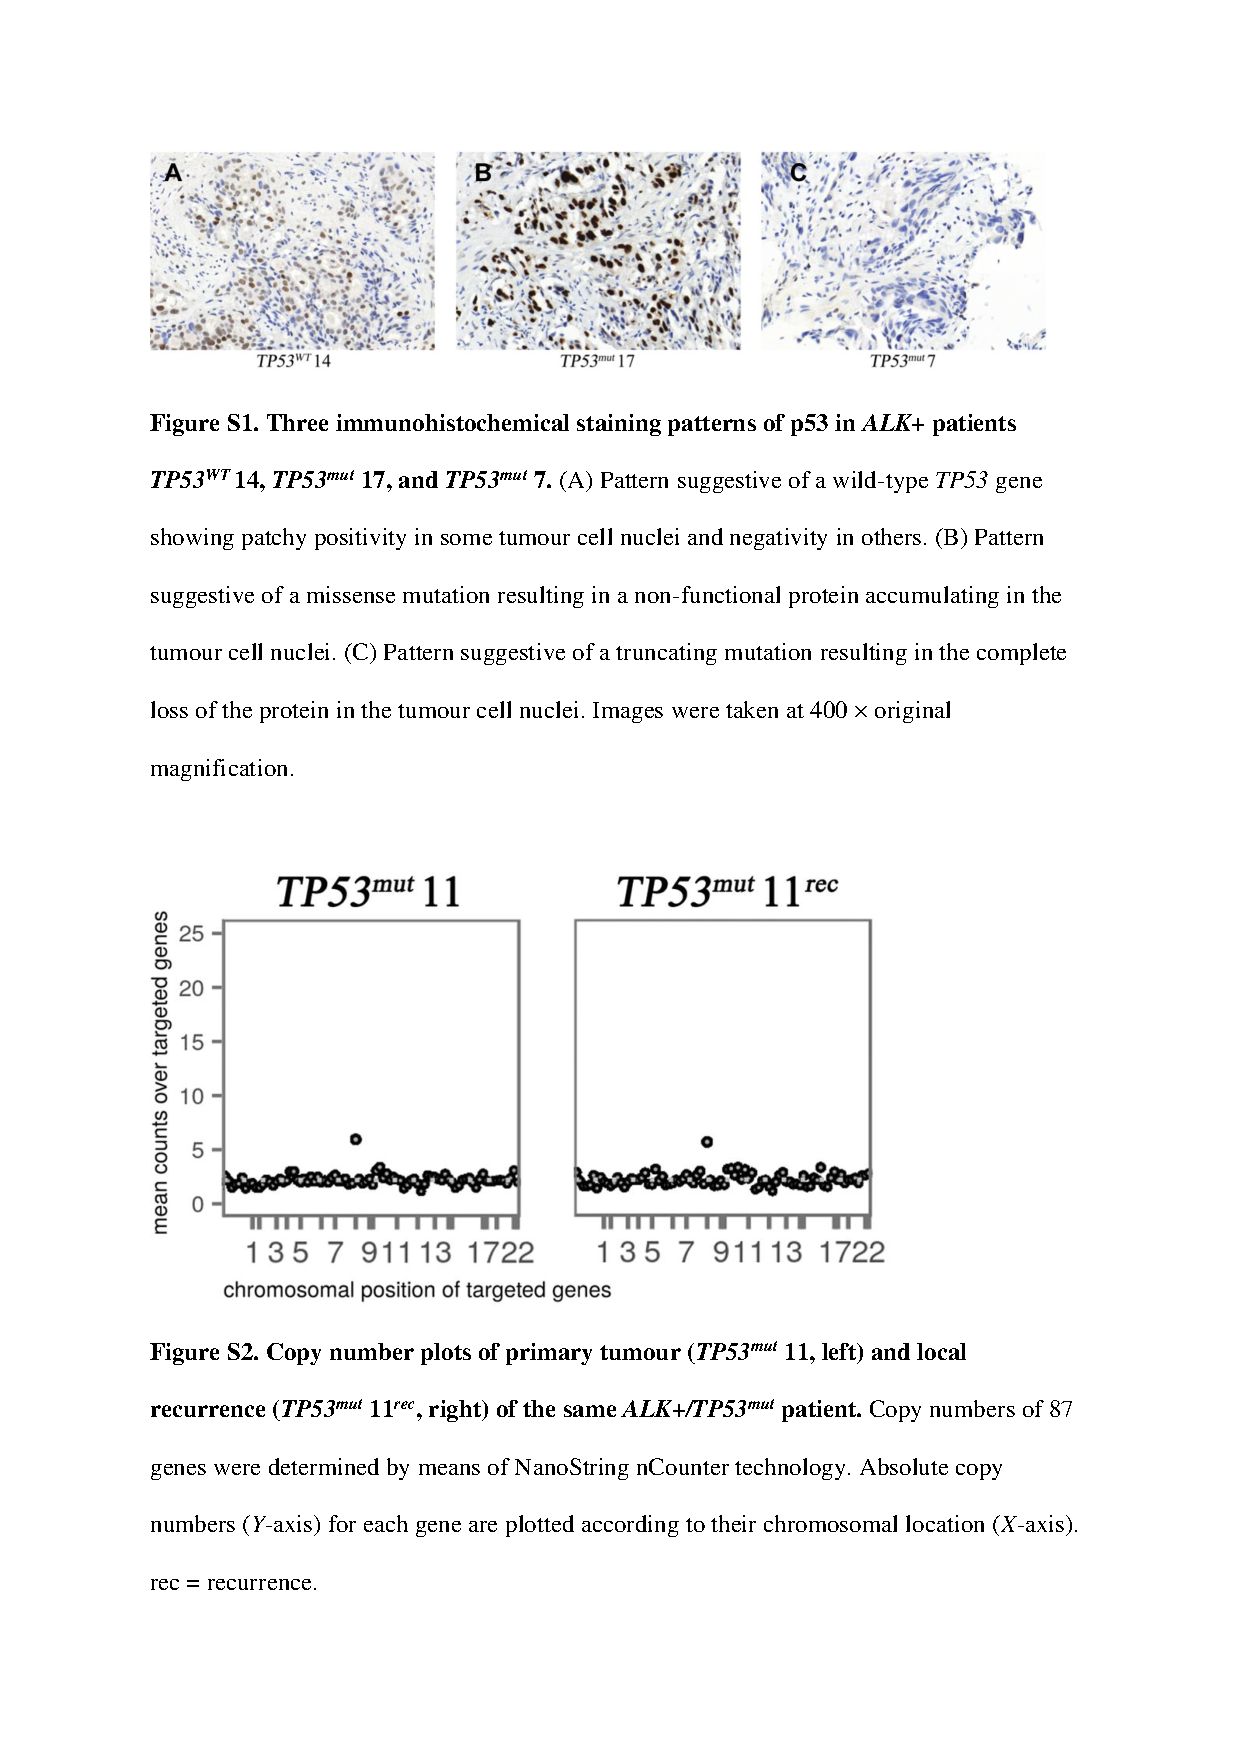
\includepdf[pages=-]{"99_Publications/Alidousty2018sup.pdf"}